% Options for packages loaded elsewhere
\PassOptionsToPackage{unicode}{hyperref}
\PassOptionsToPackage{hyphens}{url}
%
\documentclass[
]{book}
\usepackage{amsmath,amssymb}
\usepackage{iftex}
\ifPDFTeX
  \usepackage[T1]{fontenc}
  \usepackage[utf8]{inputenc}
  \usepackage{textcomp} % provide euro and other symbols
\else % if luatex or xetex
  \usepackage{unicode-math} % this also loads fontspec
  \defaultfontfeatures{Scale=MatchLowercase}
  \defaultfontfeatures[\rmfamily]{Ligatures=TeX,Scale=1}
\fi
\usepackage{lmodern}
\ifPDFTeX\else
  % xetex/luatex font selection
\fi
% Use upquote if available, for straight quotes in verbatim environments
\IfFileExists{upquote.sty}{\usepackage{upquote}}{}
\IfFileExists{microtype.sty}{% use microtype if available
  \usepackage[]{microtype}
  \UseMicrotypeSet[protrusion]{basicmath} % disable protrusion for tt fonts
}{}
\makeatletter
\@ifundefined{KOMAClassName}{% if non-KOMA class
  \IfFileExists{parskip.sty}{%
    \usepackage{parskip}
  }{% else
    \setlength{\parindent}{0pt}
    \setlength{\parskip}{6pt plus 2pt minus 1pt}}
}{% if KOMA class
  \KOMAoptions{parskip=half}}
\makeatother
\usepackage{xcolor}
\usepackage{listings}
\newcommand{\passthrough}[1]{#1}
\lstset{defaultdialect=[5.3]Lua}
\lstset{defaultdialect=[x86masm]Assembler}
\usepackage{longtable,booktabs,array}
\usepackage{calc} % for calculating minipage widths
% Correct order of tables after \paragraph or \subparagraph
\usepackage{etoolbox}
\makeatletter
\patchcmd\longtable{\par}{\if@noskipsec\mbox{}\fi\par}{}{}
\makeatother
% Allow footnotes in longtable head/foot
\IfFileExists{footnotehyper.sty}{\usepackage{footnotehyper}}{\usepackage{footnote}}
\makesavenoteenv{longtable}
\usepackage{graphicx}
\makeatletter
\def\maxwidth{\ifdim\Gin@nat@width>\linewidth\linewidth\else\Gin@nat@width\fi}
\def\maxheight{\ifdim\Gin@nat@height>\textheight\textheight\else\Gin@nat@height\fi}
\makeatother
% Scale images if necessary, so that they will not overflow the page
% margins by default, and it is still possible to overwrite the defaults
% using explicit options in \includegraphics[width, height, ...]{}
\setkeys{Gin}{width=\maxwidth,height=\maxheight,keepaspectratio}
% Set default figure placement to htbp
\makeatletter
\def\fps@figure{htbp}
\makeatother
\setlength{\emergencystretch}{3em} % prevent overfull lines
\providecommand{\tightlist}{%
  \setlength{\itemsep}{0pt}\setlength{\parskip}{0pt}}
\setcounter{secnumdepth}{5}
\usepackage{booktabs}
\usepackage{amsthm}
\usepackage{fontspec}
\setmainfont{Helvetica}
\makeatletter
\def\thm@space@setup{%
  \thm@preskip=8pt plus 2pt minus 4pt
  \thm@postskip=\thm@preskip
}
\makeatother
\renewcommand{\topfraction}{.85}
\renewcommand{\bottomfraction}{.7}
\renewcommand{\textfraction}{.15}
\renewcommand{\floatpagefraction}{.66}
\setcounter{topnumber}{3}
\setcounter{bottomnumber}{3}
\setcounter{totalnumber}{4}
\usepackage{float}
\ifLuaTeX
  \usepackage{selnolig}  % disable illegal ligatures
\fi
\usepackage[]{natbib}
\bibliographystyle{apalike}
\IfFileExists{bookmark.sty}{\usepackage{bookmark}}{\usepackage{hyperref}}
\IfFileExists{xurl.sty}{\usepackage{xurl}}{} % add URL line breaks if available
\urlstyle{same}
\hypersetup{
  pdftitle={A Practical Primer in Human Complex Genetics},
  pdfauthor={dr. Sander W. van der Laan  },
  hidelinks,
  pdfcreator={LaTeX via pandoc}}

\title{A Practical Primer in Human Complex Genetics}
\usepackage{etoolbox}
\makeatletter
\providecommand{\subtitle}[1]{% add subtitle to \maketitle
  \apptocmd{\@title}{\par {\large #1 \par}}{}{}
}
\makeatother
\subtitle{with a use-case in cardiovascular disease}
\author{\href{https://vanderlaanand.science}{dr. Sander W. van der Laan} \href{https://www.twitter.com/swvanderlaan}{
\includegraphics[width=0.02\textwidth,height=\textheight]{img/_logo/twitter_circle_blue.png}} \href{mailto:s.w.vanderlaan@gmail.com}{
\includegraphics[width=0.02\textwidth,height=\textheight]{img/_logo/email_circle_blue.png}}}
\date{Version 2.0.0 \textbar{} last update: 2024-03-25}

\begin{document}
\maketitle

{
\setcounter{tocdepth}{1}
\tableofcontents
}
\hypertarget{about-this-primer}{%
\chapter{About this primer}\label{about-this-primer}}

Ever since the first genome-wide association study (GWAS) on \href{https://doi.org/10.1126/science.1109557}{age-related macular degeneration}, and the promise of personalized medicine in the wake of the Human Genome Project, large-scale genetic association studies hold significant sway in contemporary health research and \href{http://dx.doi.org/10.1038/nrd.2017.262}{drive drug-development pipelines}. In the past 2 decades, researchers delved into GWAS, aiming to unveil genetic variations linked to both human traits, such as the color of your eyes, and rare and common complex diseases. These findings serve as crucial keys to unravel the intricate mechanisms underlying diseases, shedding light on whether the correlations identified in observational studies between risk factors and diseases are truly causal.

These studies have ushered in an exciting era where many researchers thrive on developing new methods and bioinformatic tools to parse ever-growing large datasets collected large population-based biobanks. However, the analyses of these data are challenging and it can be daunting to see the forest for tree among the many tools and their various functions. Enter \emph{A Practical Primer in Human Complex Genetics}. This \href{https://cjvanlissa.github.io/gitbook-demo/}{GitBook} was originally written back in 2022 for the \textbf{Genetic Epidemiology} course organized by the \href{https://epidemiology-education.nl}{Master Epidemiology} of Utrecht University. This practical guide will teach you how to design a GWAS, perform quality control (QC), execute the actual analyses, annotate the GWAS results, and perform further downstream post-GWAS analyses. Throughout the book you'll work with `dummy', that is fake, data, but in the end, we will use real-world data from the first release of the \href{https://www.wtccc.org.uk/ccc1/overview.html}{\emph{Welcome Trust Case-Control Consortium (WTCCC)}} focusing on coronary artery disease (CAD).

A major component of modern-day GWAS is \href{https://www.nature.com/articles/nrg2796}{genetic imputation}, but for practical reasons it is not part of this book. However, I will provide some pointers as to how to go about do this with minimal coding or scripting experience. Likewise, the courses does not cover the aspects of meta-analyses of GWAS, but some excellent resources exist to which I will direct. As this practical primer evolves, these and other topics may find their place in this book.
I should also point out that emphasis of this book is on it being a \emph{practical primer}. It is intended to provide some practical guidance to doing GWAS, and while theory is important, I will not cover this. Again, some very useful and excellent work exists to which I will point you, but I really want you to learn - and understand the theory - by \emph{doing}.

So, although originally crafted as a companion for the course, this practical guide stands on its own as a comprehensive resource for diving into all facets of doing a GWAS --- save for experimental follow-up, of course 😉.

I can imagine this seems overwhelming, but trust me, you'll be okay. Just follow this practical. You'll learn by doing and at the end of the day, you can execute a GWAS independently.

\textbf{Ready to start?}

Your first point of action is to prepare your system for this course in Chapter @ref(02\_1\_somebackgroundreading).

\hypertarget{some-background-reading}{%
\chapter{Some background reading}\label{some-background-reading}}

Standing on the shoulders of giants, that's what this book and I do. I want to acknowledge some great work that has helped me tremendously and, really, this book wouldn't exist without this awesome work. So, I do want to give you some background reading. Is it a prerequisite? No, not really. For starters, the course covers most and you'll learn as you go. And if you didn't come here through the course, you'll be fine just the same. That said, it's a always good idea to get familiar with these works as you move forward on your path towards your first GWAS - in fact, I had these printed out with markings and writings all over them as I executed my first GWAS, and they've been great as a reference many times after.

Large parts of this work are based on four awesome Nature Protocols from the \href{https://www.well.ox.ac.uk/research/research-groups/zondervan-group}{Zondervan group} at the Wellcome Center Human Genetics.

\begin{enumerate}
\def\labelenumi{\arabic{enumi}.}
\tightlist
\item
  \href{https://www.ncbi.nlm.nih.gov/pubmed/17947991}{Zondervan KT \emph{et al.} \emph{Designing candidate gene and genome-wide case-control association studies.} Nat Protoc 2007.}
\item
  \href{https://www.ncbi.nlm.nih.gov/pubmed/19390530}{Pettersson FH \emph{et al.} \emph{Marker selection for genetic case-control association studies.} Nat Protoc 2009.}
\item
  \href{https://www.ncbi.nlm.nih.gov/pubmed/21085122}{Anderson CA \emph{et al.} \emph{Data QC in genetic case-control association studies.} Nat Protoc 2010.}
\item
  \href{https://www.ncbi.nlm.nih.gov/pubmed/21293453}{Clarke GM \emph{et al.} \emph{Basic statistical analysis in genetic case-control studies.} Nat Protoc 2011.}
\end{enumerate}

An update on the community standards of QC for GWAS can be found here:

\begin{enumerate}
\def\labelenumi{\arabic{enumi}.}
\tightlist
\item
  \href{https://www.ncbi.nlm.nih.gov/pubmed/20718045}{Laurie CC \emph{et al.} \emph{Quality control and quality assurance in genotypic data for genome-wide association studies.} Genet Epidemiol 2010.}
\end{enumerate}

With respect to imputation and meta-analyses of GWAS you should also get familiar with the following two works:

\begin{enumerate}
\def\labelenumi{\arabic{enumi}.}
\tightlist
\item
  \href{https://doi.org/10.1038/nrg2796}{Marchini, J. and Howie, B. \emph{Genotype imputation for genome-wide association studies.} Nat Rev Genet 2010}
\item
  \href{https://www.ncbi.nlm.nih.gov/pubmed/18852200}{de Bakker PIW \emph{et al.} \emph{Practical aspects of imputation-driven meta-analysis of genome-wide association studies.} Hum Mol Genet 2008.}
\item
  \href{https://www.ncbi.nlm.nih.gov/pubmed/24762786}{Winkler TW \emph{et al.} \emph{Quality control and conduct of genome-wide association meta-analyses.} Nat Protoc 2014.}
\end{enumerate}

\textbf{Are you ready?}

Are you ready? Did you bring coffee and a good dose of energy? Let's start! Your first point of action is to prepare your system for this course in Chapter @ref(02\_2\_prerequisites).

\hypertarget{prerequisites}{%
\chapter{Prerequisites}\label{prerequisites}}

\hypertarget{linux-macos-and-windows}{%
\section{Linux, macOS, and Windows}\label{linux-macos-and-windows}}

Most programs made to execute genetic epidemiology studies are developed for the Unix environment, for example Linux and macOS. So, they may not work as intended in a Windows environment. Windows does allow users to install a linux subsystem within Windows 10 and you can find the detail \href{https://docs.microsoft.com/en-us/windows/wsl/about}{guide} here.

However, I highly recommend one of two options. One, install a linux subsystem on your Windows computer (for example \href{https://blog.storagecraft.com/the-dead-simple-guide-to-installing-a-linux-virtual-machine-on-windows/}{a virtual machine with Ubuntu could work}). Two, switch to macOS in combination with \href{https://brew.sh}{homebrew}. This will give you all the flexibility to use Unix-based programs for your genetic epidemiology work and at the same time you'll keep the advantage of a powerful computer with a user-friendly interface.

\begin{quote}
For this practical every command is intended for Linux/macOS, in other words Unix-systems.
\end{quote}

\hypertarget{programs-you-need}{%
\section{Programs you need}\label{programs-you-need}}

You need few programs for this practical, or for your (future) genetic epidemiology work for that matter (Table \ref{tab:programs}).

\begin{table}

\caption{\label{tab:programs}Programs needed for genetic epidemiology.}
\centering
\begin{tabular}[t]{l|l|l}
\hline
Program & Link & Description\\
\hline
PLINK & https://www.cog-genomics.org/plink2/ & PLINK is a free, open-source genetic analysis tool set, designed to perform a range of basic data parsing and quality control, as well as basic and large-scale analyses in a computationally efficient manner.\\
\hline
R & https://cran.r-project.org/ & A program to perform statistical analysis and visualizations.\\
\hline
RStudio & https://www.rstudio.com & A user-friendly R-wrap-around for code editing, debugging, analyses, and visualization.\\
\hline
Homebrew & https://brew.sh & A great extension for Mac-users to install really useful programs that Apple didn't.\\
\hline
\end{tabular}
\end{table}

\hypertarget{rstudio}{%
\subsection{RStudio}\label{rstudio}}

RStudio is a very user-friendly interface around R that makes your R-scripting-life a lot easier. You should get used to that.
We have a clean installation of Ubuntu in our VirtualMachine with full administrator rights. Let's start by installing RStudio. On your VirtualMachine go to the website of \href{https://www.rstudio.com/products/rstudio/download/\#download}{RStudio} and select the right installer (\passthrough{\lstinline!Ubuntu 18+/Debian 10+!}), it should be name something like \passthrough{\lstinline!rstudio-2022.02.1-461-amd64.deb!}.

Double click the file after download (it's probably on the Desktop or the Download folder) and follow the instructions.

RStudio comes with R so you don't have to worry about that.

\hypertarget{plink}{%
\subsection{PLINK}\label{plink}}

Right, onto PLINK.

All genetic analyses can be done in PLINK, even on your laptop, but with large datasets, for example \href{https://www.ukbiobank.ac.uk}{UK Biobank} size, it is better to switch to a \href{https://en.wikipedia.org/wiki/High-performance_computing}{high-performance computing cluster} like we have available at the \href{https://wiki.bioinformatics.umcutrecht.nl/bin/view/HPC/WebHome}{Utrecht Science Park}. The original PLINK v1.07 can be found \href{https://zzz.bwh.harvard.edu/plink/index.shtml}{here}, but nowadays we are using a newer, faster version: PLINK v1.9 which can be found \href{https://www.cog-genomics.org/plink2}{here}. It still says `PLINK 1.90 beta' but you can consider this version stable and save to work with, but as you can see, some functions are not supported anymore.

You should be downloading the Linux 64-bits version indicated with the blue arrow in Figure \ref{fig:plink}

\begin{figure}

{\centering 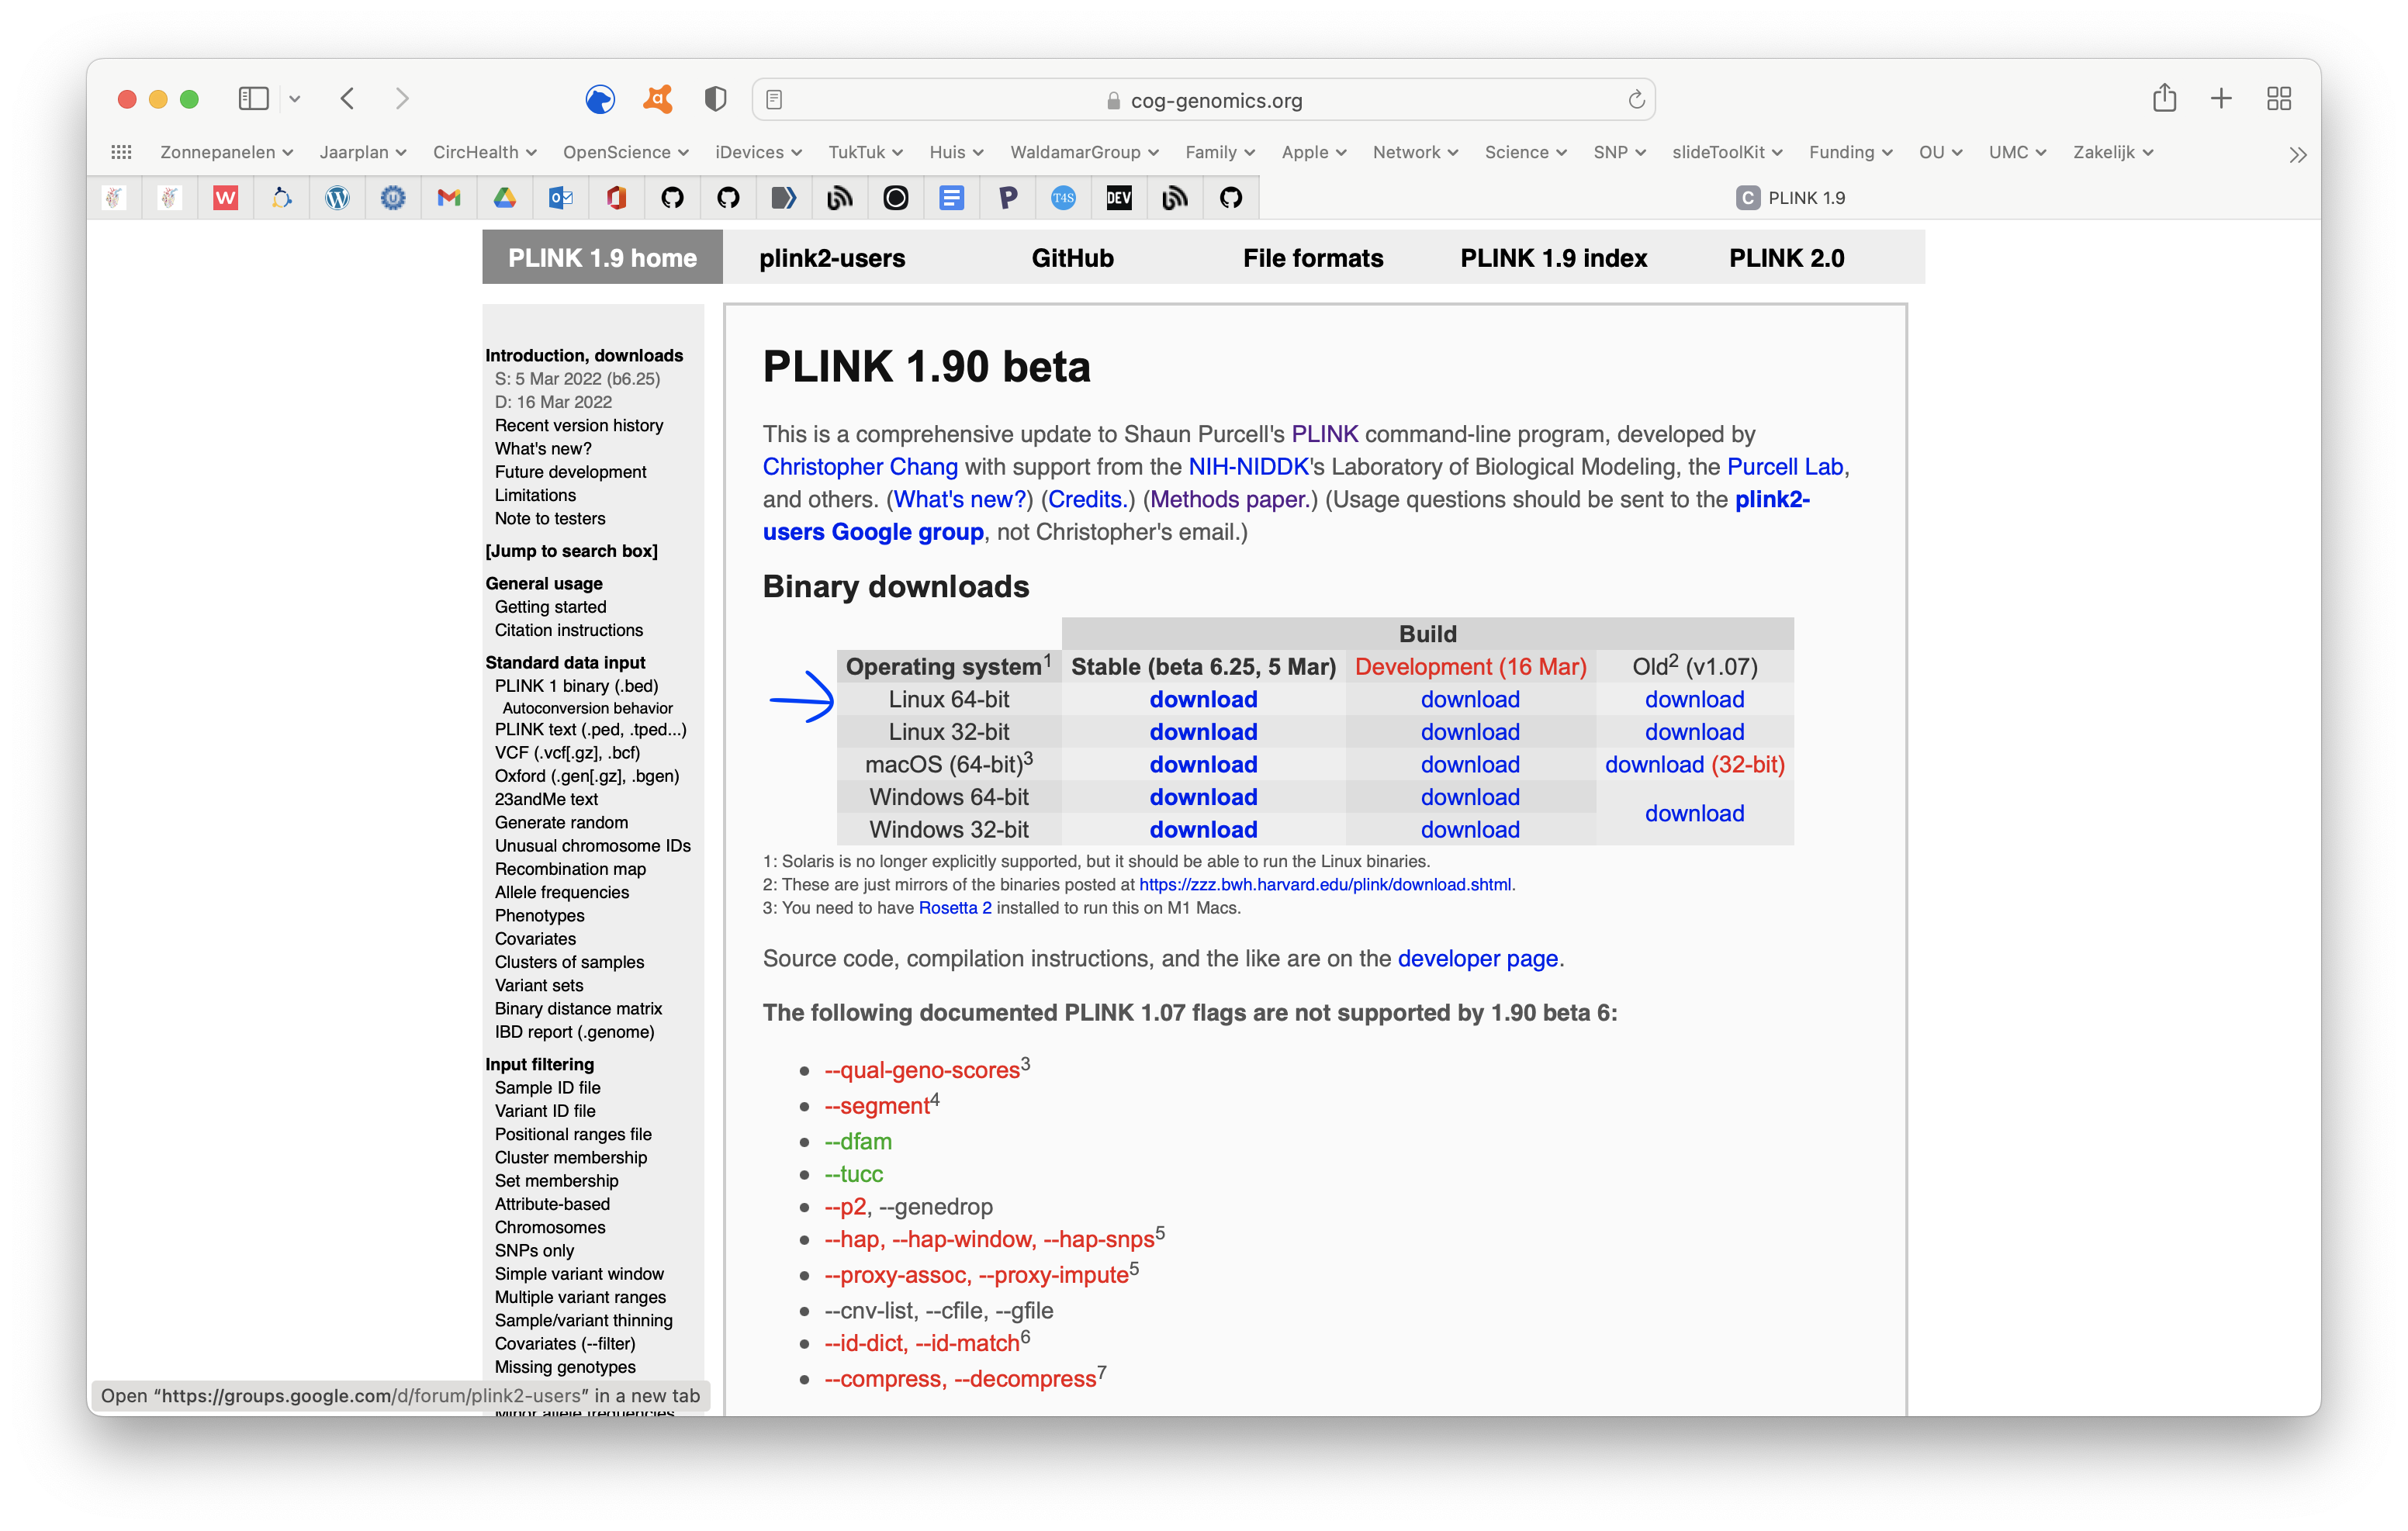
\includegraphics[width=43.11in]{img/plink} 

}

\caption{The PLINK v1.9 website.}\label{fig:plink}
\end{figure}

You'll download a zip-file containing PLINK to the Downloads folder, or the Desktop. If all is fine, you should be able to double click the \passthrough{\lstinline!.zip!}-file and it will unpack there and then.

\hypertarget{alternatives-to-plink}{%
\subsection{Alternatives to PLINK}\label{alternatives-to-plink}}

Nowadays, a lot of people also use programs like \href{snptest}{SNPTEST}, \href{https://data.broadinstitute.org/alkesgroup/BOLT-LMM/}{BOLT-LMM}, \href{http://cnsgenomics.com/software/gcta/\#Overview}{GCTA}, or \href{https://rgcgithub.github.io/regenie/}{regenie} as alternatives to execute GWAS and downstream analyses, for example heritability estimation, Fst-calculation, and so on.

\hypertarget{other-programs}{%
\subsection{Other programs}\label{other-programs}}

Mendelian randomization can be done either with the \href{http://cnsgenomics.com/software/smr/\#Overview}{SMR} or \href{http://cnsgenomics.com/software/gsmr/}{GSMR} function from GCTA, or with R-packages, like \href{https://mrcieu.github.io/TwoSampleMR/}{\passthrough{\lstinline!TwoSampleMR!}}.

\hypertarget{the-terminal}{%
\section{The Terminal}\label{the-terminal}}

For all the above programs, except RStudio, you will need the \passthrough{\lstinline!Terminal!}. This comes with every major operating system; on Windows it is called `PowerShell', but let's not go there. And regardless, you will (have to start to) make your own scripts. The benefit of using scripts is that each step in your workflow is clearly stipulated and annotated, and it allows for greater reproducibility, easier troubleshooting, and scaling up to high-performance computer clusters.

Open the terminal, it should be on the left in the toolbar as a little black computer-monitor-like icon. Mac users can type \passthrough{\lstinline!command + space!} and type \passthrough{\lstinline!terminal!}, a terminal screen should open.

\begin{quote}
From now on we will use little code blocks like the example to indicate a code you should type/copy-paste and hit enter. If a code is followed by a comment, it is indicated by a \# - you don't need to copy-paste and execute this.
\end{quote}

\begin{lstlisting}
CODE BLOCK

CODE BLOCK # some comment here
\end{lstlisting}

\hypertarget{the-data-you-need}{%
\subsection{The data you need}\label{the-data-you-need}}

Now, pay attention. If you came here through the course \textbf{Genetic Epidemiology}, you don't have to do anything. All the data you need are already downloaded.

However, when you are using this book as a standalone, you'll need to start by downloading the data you need for this practical to your Desktop.

Here's the link to the data.

\href{https://drive.google.com/drive/folders/1iDLB1y534DfgEZNPCYBrIj5X7g_XlBba?usp=share_link}{Link to Google Drive with data}

Make sure you put the data in the \passthrough{\lstinline!\~/Desktop/practical/!} folder.

Alternatively, you could download this through some Terminal commands. This will create a directory on your Desktop with the command \passthrough{\lstinline!mkdir!}. The \passthrough{\lstinline!-v!} flag indicates the program should be \emph{verbose}, meaning it should tell you what it is doing. And it will automagically download the data to the right folder.

\begin{lstlisting}
mkdir -v ~/Desktop/practical/

wget https://drive.google.com/drive/folders/1iDLB1y534DfgEZNPCYBrIj5X7g_XlBba?usp=share_link -P ~/Desktop/practical/
\end{lstlisting}

The data are pretty large (approx. 15Gb), so this will take a minute or two depending on your internet connection. Time to stretch your legs or grab a coffee (data scientists don't drink tea).

\hypertarget{navigating-the-terminal}{%
\subsection{Navigating the Terminal}\label{navigating-the-terminal}}

You can navigate around the computer through the terminal by typing \passthrough{\lstinline!cd <path>!}; \passthrough{\lstinline!cd!} stands for ``change directory'' and means ``some\_file\_directory\_you\_want\_to\_go\_to''.

\textbf{For Linux/macOS Users}

\emph{will bring you to your home directory}

\begin{lstlisting}
cd ~ 
\end{lstlisting}

\emph{will bring you to the parent directory (up one level) }

\begin{lstlisting}
cd ../ 
\end{lstlisting}

\emph{will bring you to the XXX directory}

\begin{lstlisting}
cd XXX 
\end{lstlisting}

Let's navigate to the folder you just downloaded.

\begin{lstlisting}
cd ~/Desktop/practical
\end{lstlisting}

Let's check out what is inside the directory, by listing (\passthrough{\lstinline!ls!}) its contents.

\begin{lstlisting}
ls -lh
\end{lstlisting}

\textbf{For Linux/macOS Users}

\emph{shows files as list}

\begin{lstlisting}
ls -l 
\end{lstlisting}

\emph{shows files as list with human readable format }

\begin{lstlisting}
ls -lh 
\end{lstlisting}

\emph{shows the files as list sorted by time edited}

\begin{lstlisting}
ls -lt 
\end{lstlisting}

\emph{shows the files as list sorted by size}

\begin{lstlisting}
ls -lS 
\end{lstlisting}

Adding the flags \passthrough{\lstinline!-lh!} will get you the contents of a directory in a list (\passthrough{\lstinline!-l!}) and make the size `human-readable' (\passthrough{\lstinline!-h!}).

You can also count the number of files.

\begin{lstlisting}
ls | wc -l
\end{lstlisting}

And if you want to know all the function of a program simply type the following.

\begin{lstlisting}
man ls
\end{lstlisting}

This will take you to a manual of the program with an extensive description of each flag (Figure \ref{fig:ls-manual}).

\begin{figure}

{\centering 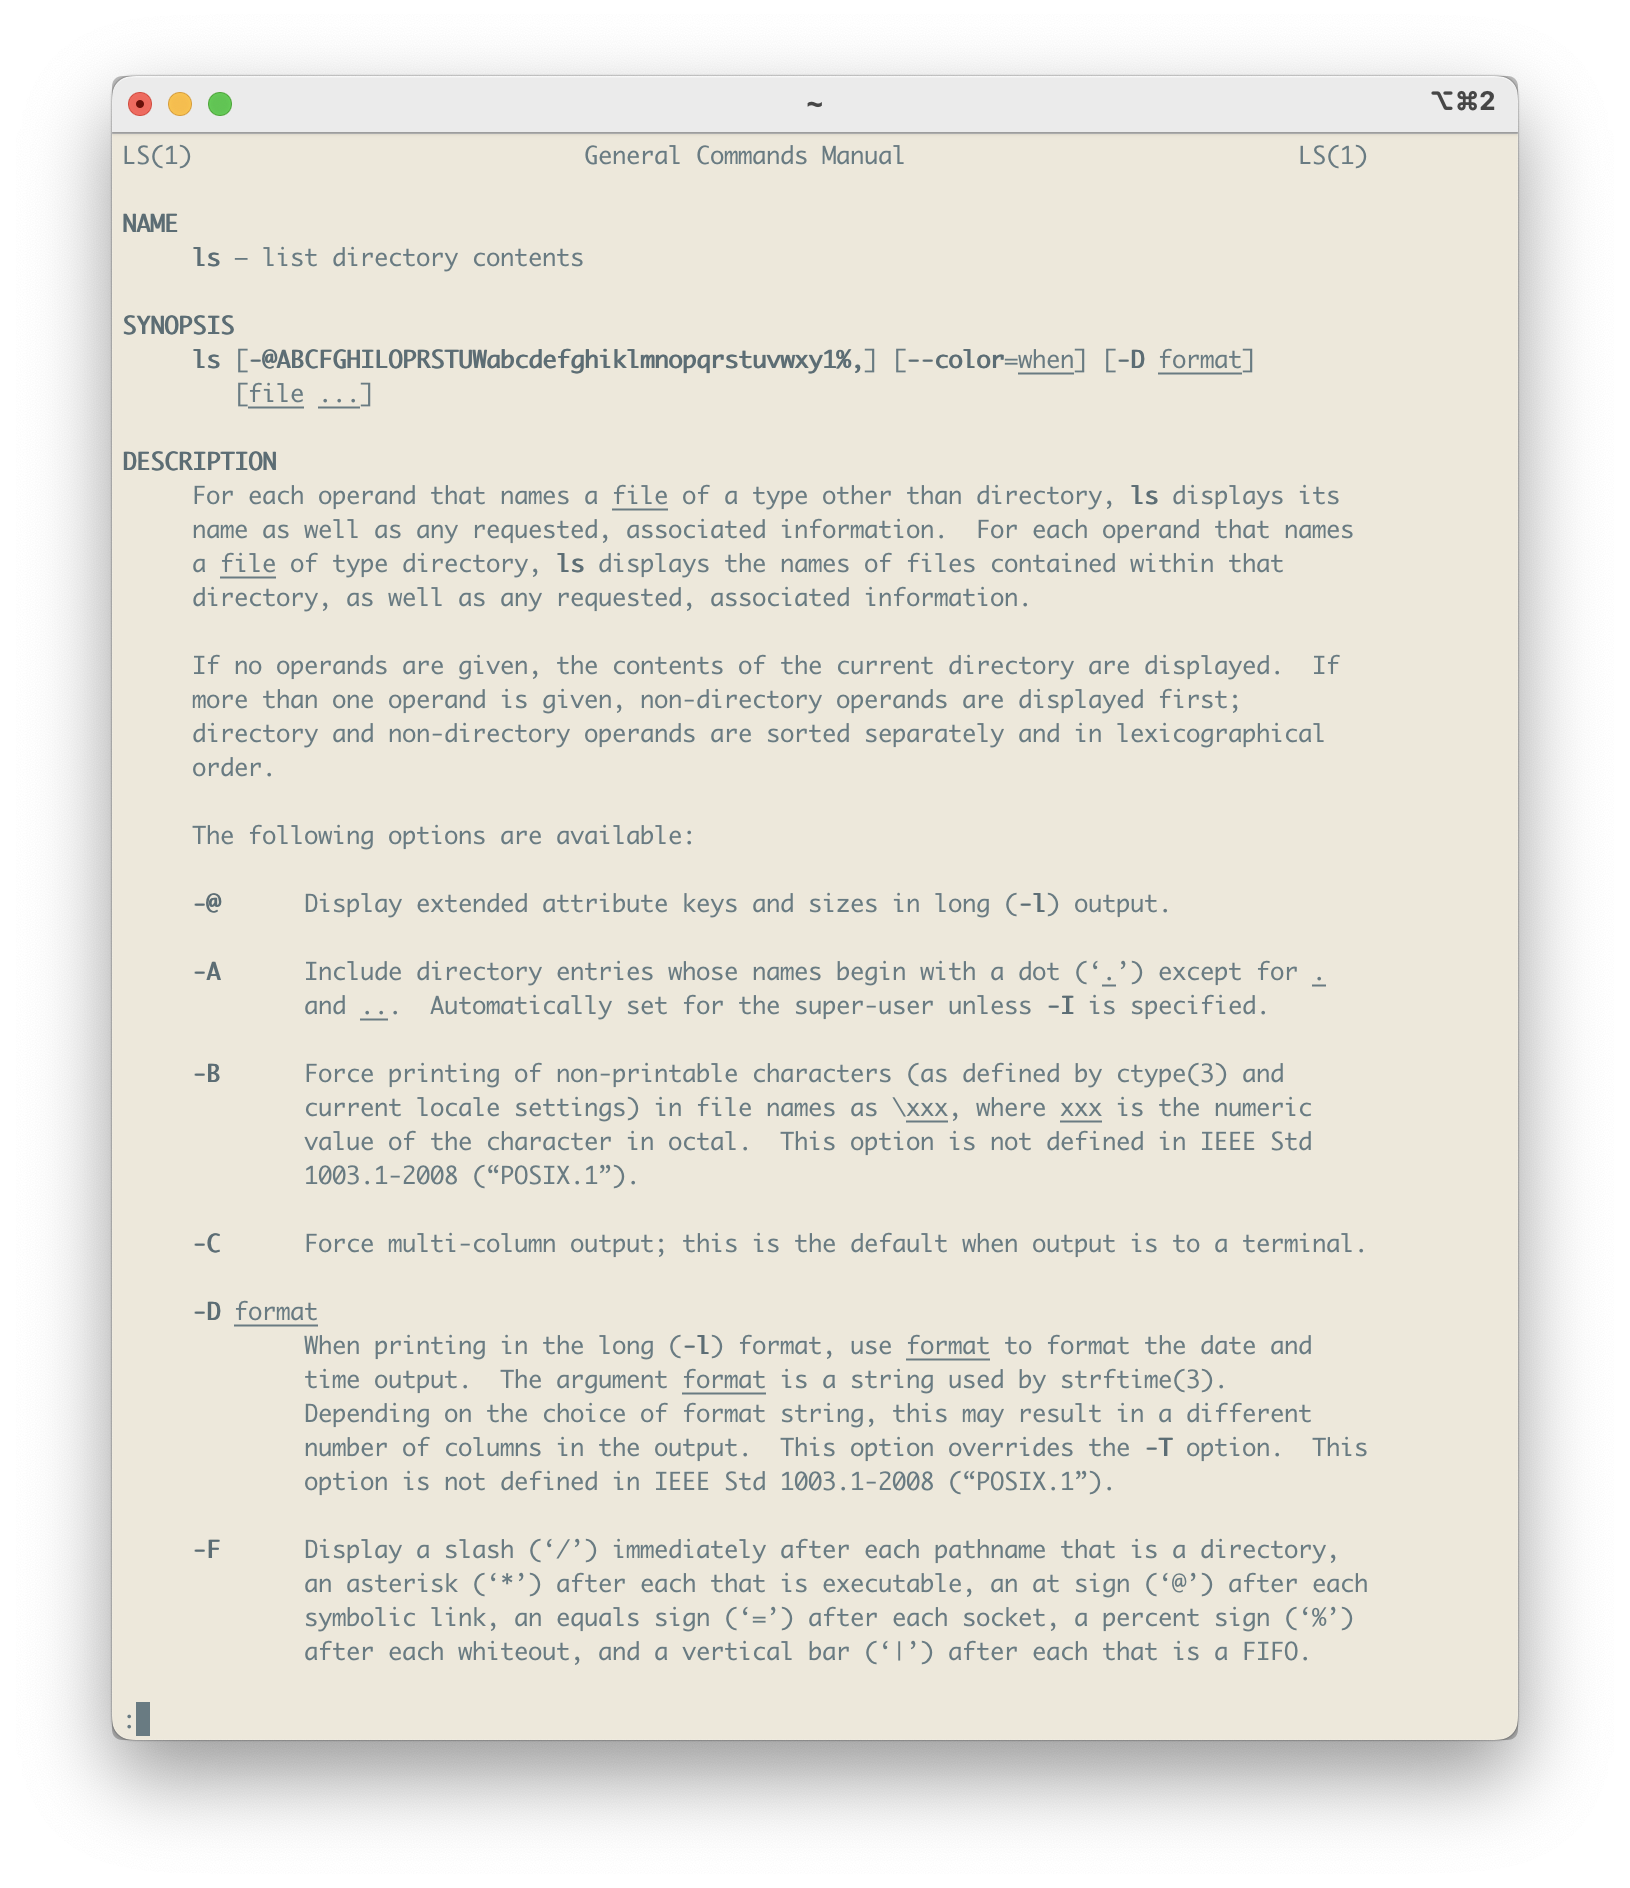
\includegraphics[width=22.64in]{img/ls_manual} 

}

\caption{Partial output from the ls-manual.}\label{fig:ls-manual}
\end{figure}

We also want to copy \passthrough{\lstinline!plink!} to that practical folder.

\begin{lstlisting}
cp -v ~/Downloads/plink/plink ~/Desktop/practical/plink 
\end{lstlisting}

\hypertarget{installing-some-r-packages}{%
\section{Installing some R packages}\label{installing-some-r-packages}}

For the course we set up a CoCalc Server and everything should be fine; we installed everything you need.

If you are using this as a standalone book, you'll need to install some things. For certain \passthrough{\lstinline!r!}-packages, we need to install some additional software on your operating system. Depending on your system, type the following and just follow the instructions in the Terminal:

\textbf{For Linux/macOS Users}

\begin{lstlisting}
sudo apt-get install libcurl4 libcurl4-openssl-dev -y

sudo apt-get install libssl-dev
\end{lstlisting}

\textbf{For macOS Users}

Just follow the instructions in the Terminal.

Start by installing \href{https://brew.sh}{\passthrough{\lstinline!brew!}}.

\begin{lstlisting}
/bin/bash -c "$(curl -fsSL https://raw.githubusercontent.com/Homebrew/install/HEAD/install.sh)"
\end{lstlisting}

\begin{lstlisting}
brew install --cask rstudio
brew install r
\end{lstlisting}

Now close the terminal window - really make sure that the terminal-program has quit.

Open your fresh installation of RStudio by double clicking the icon. You should be seeing something like figure \ref{fig:rstudio-screenshot}

\begin{figure}

{\centering 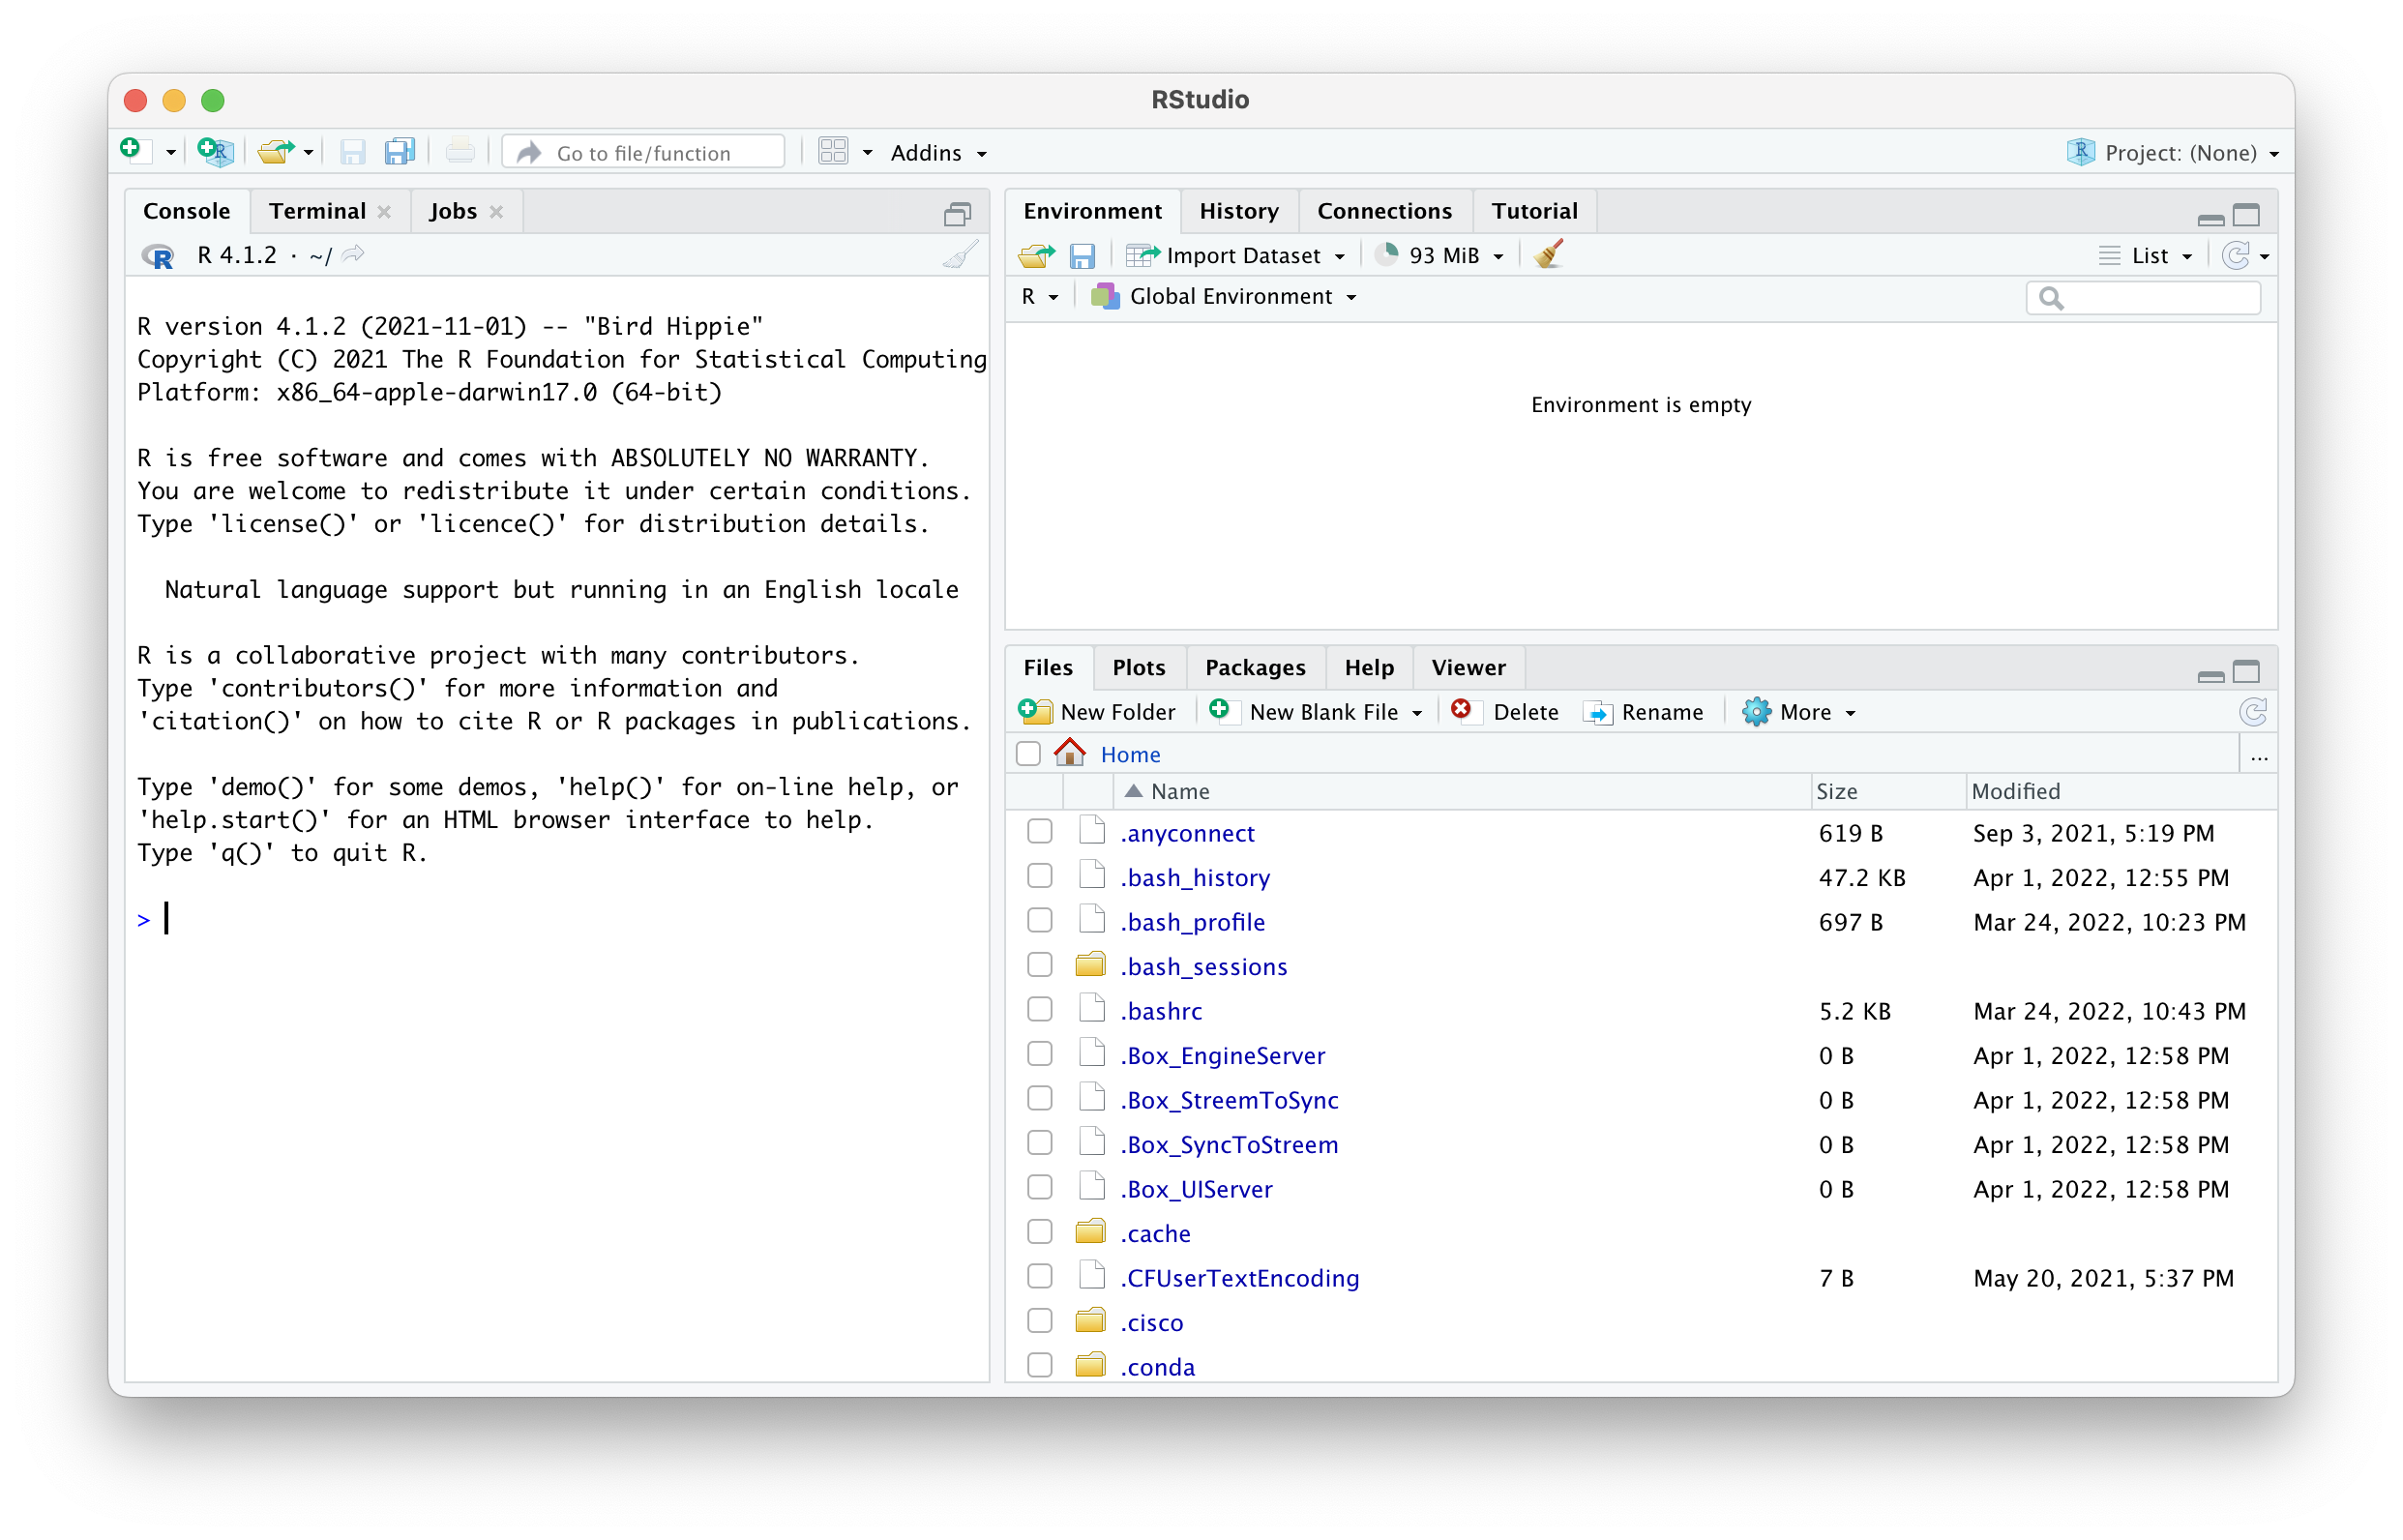
\includegraphics[width=34.5in]{img/rstudio-screenshot} 

}

\caption{RStudio screenshot.}\label{fig:rstudio-screenshot}
\end{figure}

In the top right, you see a little green-white plus-sign, click this and select `R Notebook' (Figure \ref{fig:rstudio-screenshot-create-notebook}).

\begin{figure}

{\centering 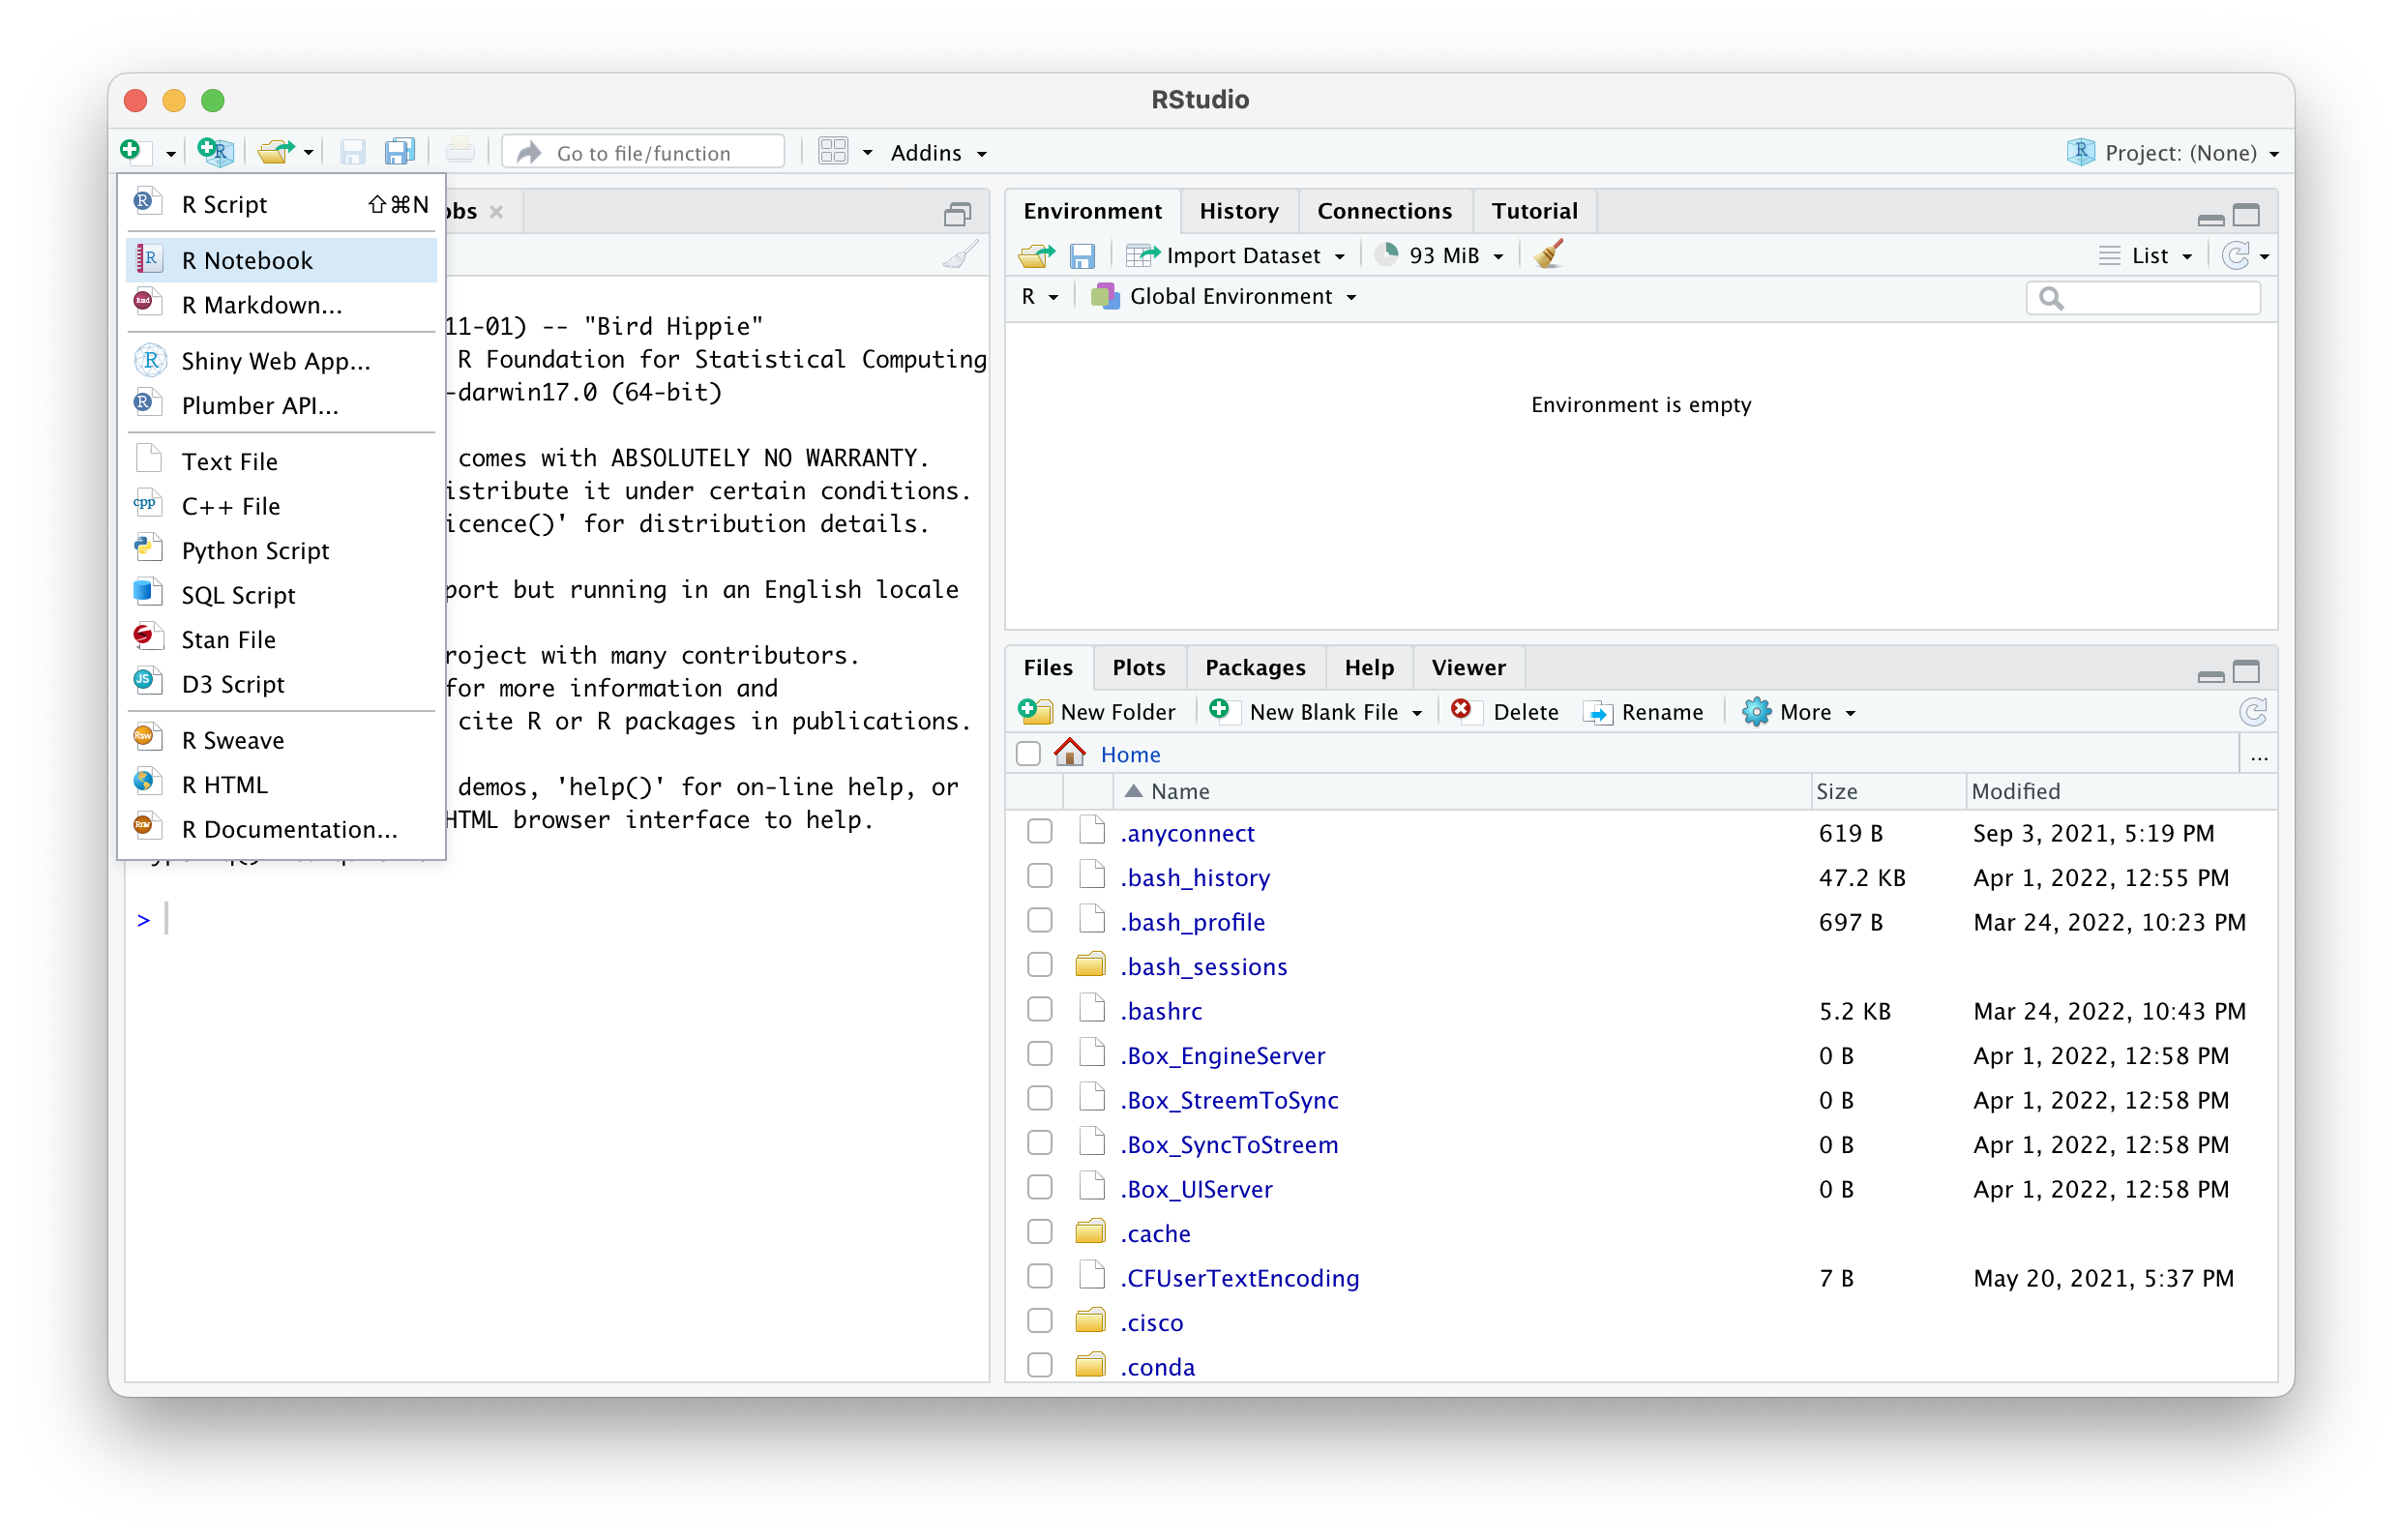
\includegraphics[width=34.5in]{img/rstudio-screenshot-create-notebook} 

}

\caption{RStudio screenshot.}\label{fig:rstudio-screenshot-create-notebook}
\end{figure}

You will create an untitled (\passthrough{\lstinline!Untitled1!}) \passthrough{\lstinline!R!} notebook: you can combine text descriptions, like you would in a lab-journal, with code-sections. Read what is in the notebook to get a grasp on that (Figure \ref{fig:rstudio-screenshot-notebook}).

\begin{figure}

{\centering 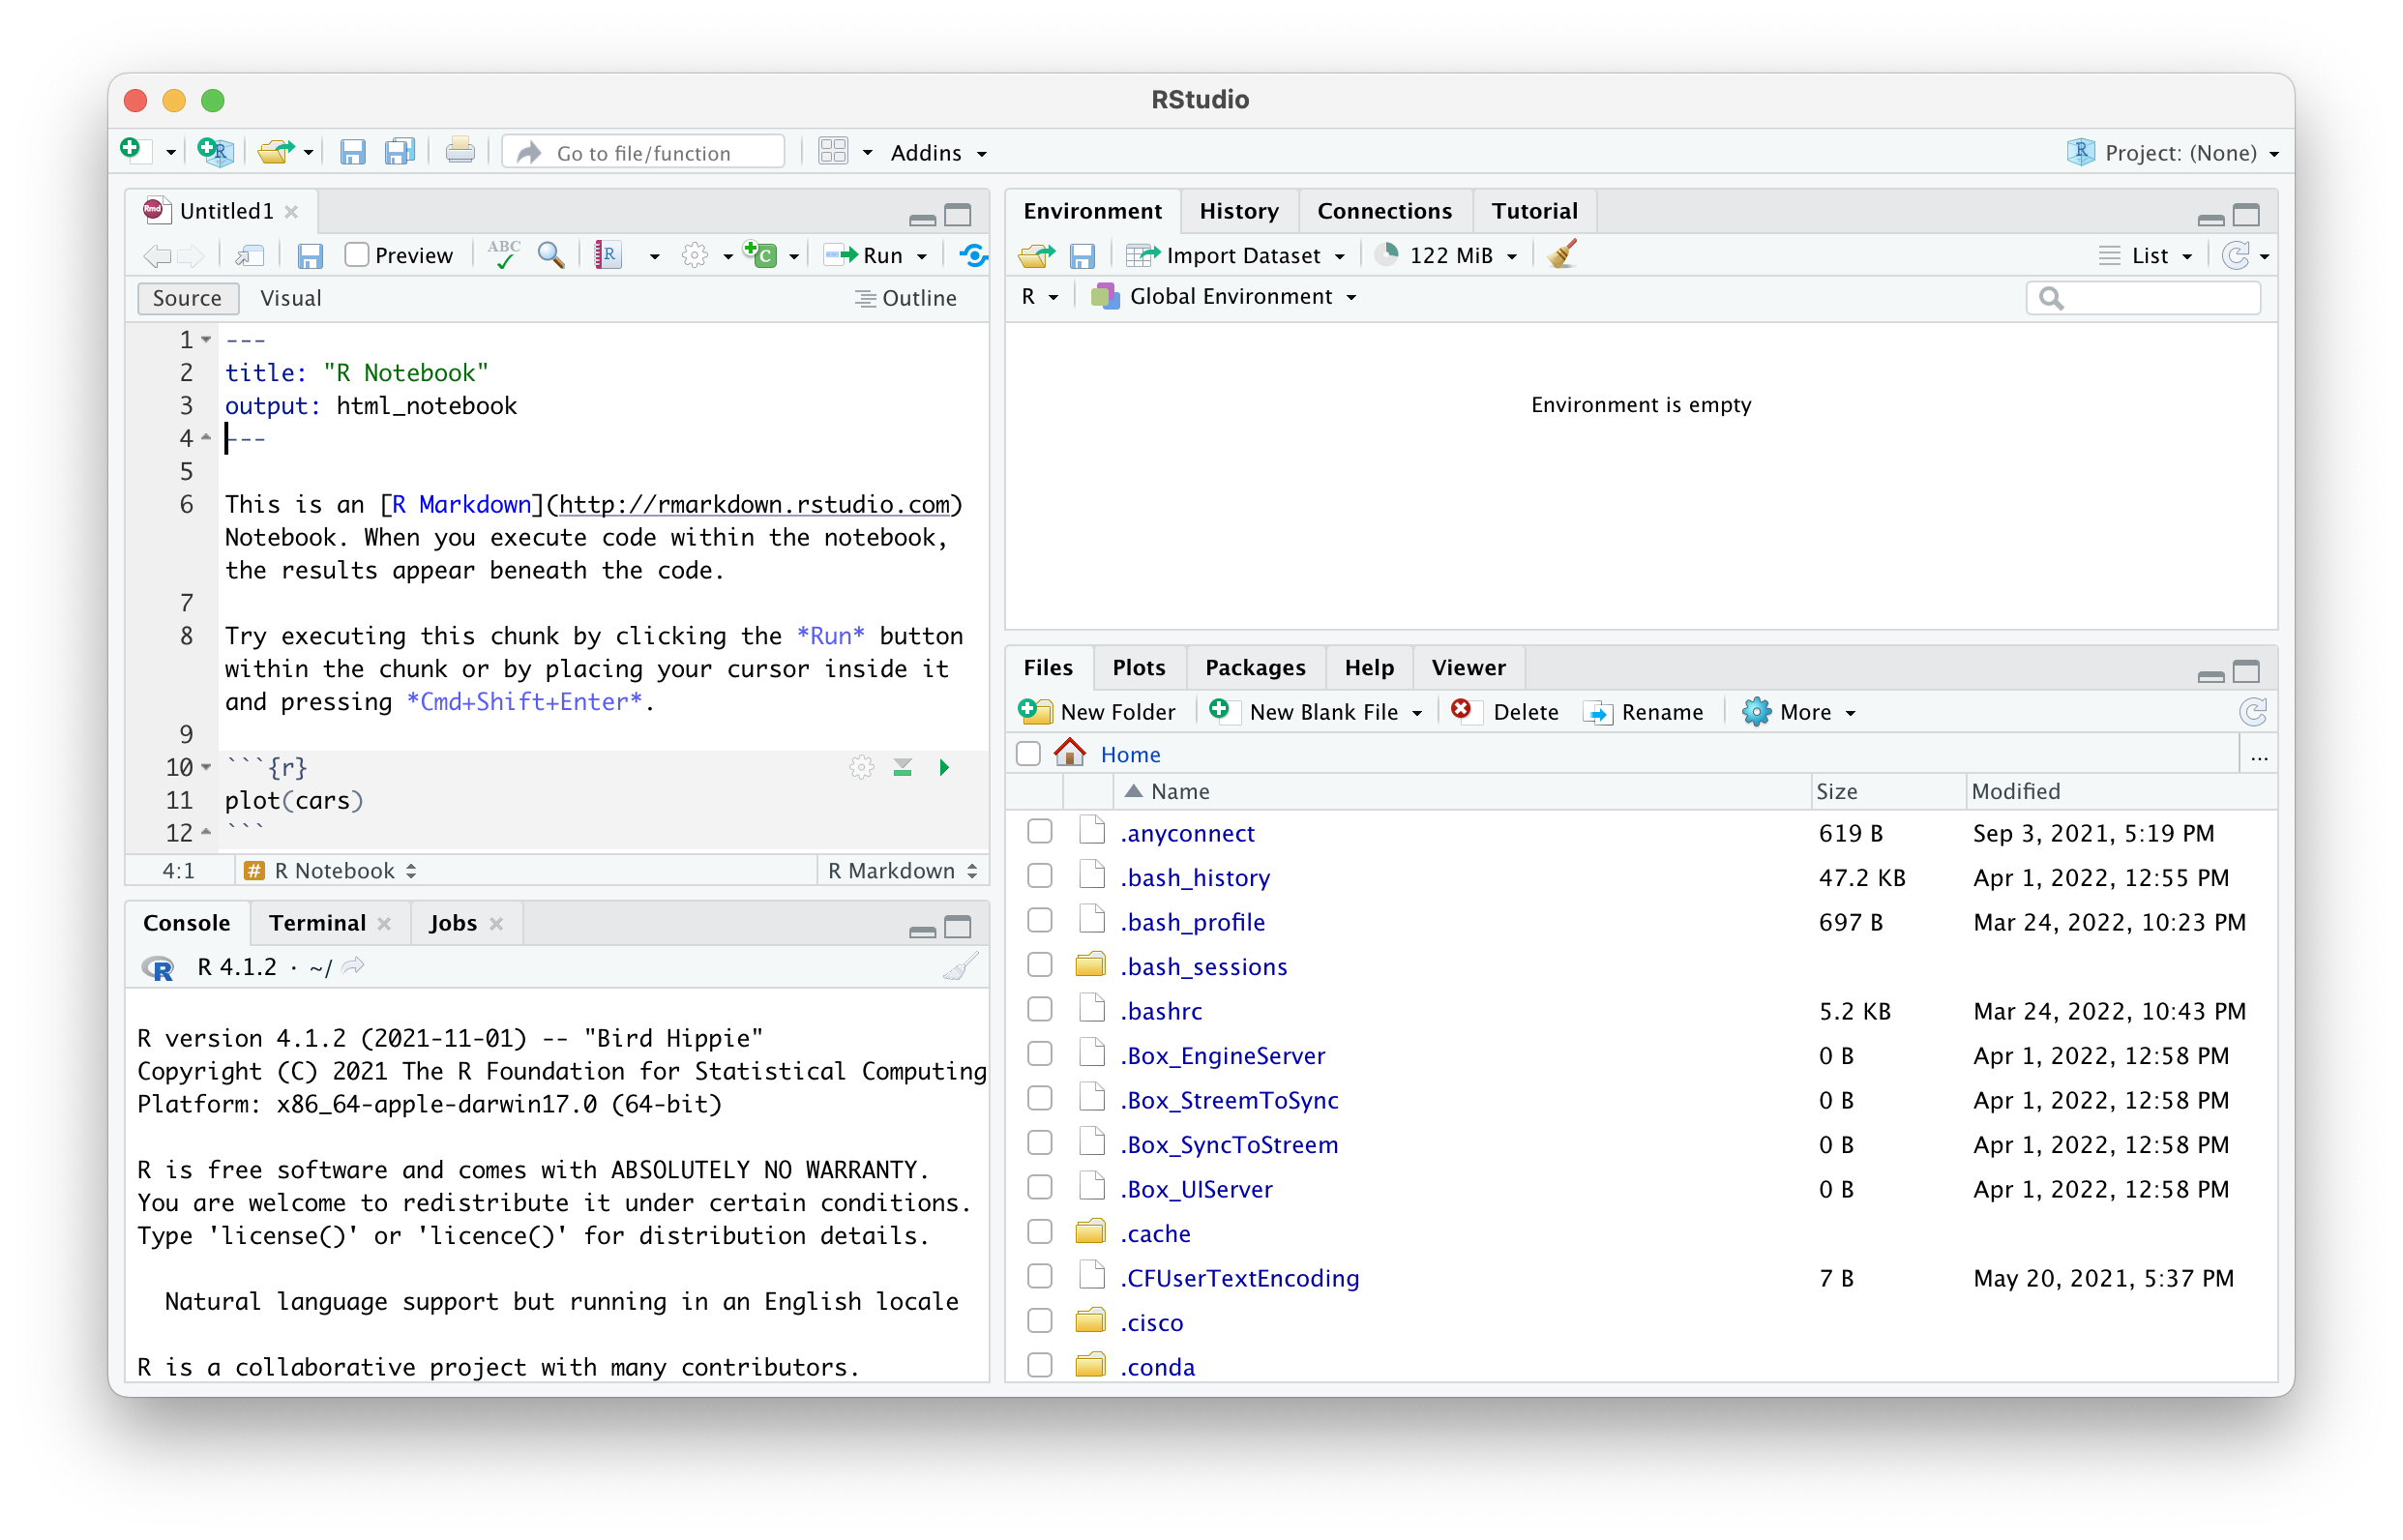
\includegraphics[width=34.5in]{img/rstudio-screenshot-notebook} 

}

\caption{RStudio screenshot.}\label{fig:rstudio-screenshot-notebook}
\end{figure}

Right, you should be installing some packages. To do so, you can remove \passthrough{\lstinline!plot(cars)!} (or leave and create a new code-block as per instructions in the notebook), and copy paste the code below.

\begin{lstlisting}[language=R]
install.packages(c("httr", "usethis", "data.table", "devtools", 
                   "qqman", "CMplot", "plotly", 
                   "dplyr", "tibble", "openxlsx"))
devtools::install_github("kassambara/ggpubr")
devtools::install_github("oliviasabik/RACER")
\end{lstlisting}

You should load these packages too.

\begin{lstlisting}[language=R]
library("ggpubr")
library("httr")
library("usethis")
library("data.table")
library("devtools")
library("qqman")
library("CMplot")
library("tibble")
library("plotly")
library("dplyr")
library("openxlsx")
library("RACER")
\end{lstlisting}

All in all this may take some time, good moment to relax, review your notes, stretch your legs, or take a coffee.

\hypertarget{are-you-ready}{%
\section{Are you ready?}\label{are-you-ready}}

Are you ready? Did you bring coffee and a good dose of energy? Let's start!

Oh, one more thing: you can save your notebook, the one you just created, to keep all the \passthrough{\lstinline!R!} codes you are applying in the next chapters and add descriptions and notes. If you save this notebook you'll notice that a \passthrough{\lstinline!html!}-file is created. This file is a legible webbrowser-friendly version of your work and contains the codes and the output (code messages, tables, and figures). And the nice thing is, that you can easily share it with others over email.

\hypertarget{epilogue}{%
\chapter{Epilogue}\label{epilogue}}

What started as a simple `let's write a practical on how to do a GWAS', escalated into this GitBook. My second book. My fifth child (as far as I know). I hope you found it to be useful and learned a bit.

That said, much can be improved and so don't hesitate to contact me.

As with any proper epilogue I should not forget a heartfelt and honest thank you to the readers and users of this work. Gratitude also goes to my dear colleagues Charlotte Onland, Jessica van Setten, and Kristel van Eijk, and former colleague Sara Pulit who asked me back in 2017 to join the course as a lecturer. It has been a pleasure to work with and learn from you, and it has been a fun (and sometimes stressful) experience to teach this course.

\hypertarget{todo}{%
\chapter{Things to do}\label{todo}}

I provide a list of things to do, to improve, to alter, to edit or to add. Crazy ideas. Useful tips, tricks, or links.

Obviously this list is not exhaustive nor intended for practical use for anyone else but me.

\hypertarget{moscow}{%
\section{MoSCoW}\label{moscow}}

List of to-do's according to MoSCoW: \emph{must have}, \emph{should have}, \emph{could have}, \emph{would have}.

\hypertarget{contents}{%
\subsection{Contents}\label{contents}}

\begin{itemize}
\tightlist
\item[$\boxtimes$]
  \passthrough{\lstinline!M!} add in full installation instructions for UBUNTU
\item
  {[}{]} \passthrough{\lstinline!M!} add in full installation instructions for macOS
\item
  {[}{]} \passthrough{\lstinline!M!} conditional analysis
\item
  {[}{]} \passthrough{\lstinline!M!} statistical finemapping
\item[$\boxtimes$]
  \passthrough{\lstinline!M!} regional association plotting
\item
  {[}{]} \passthrough{\lstinline!M!} colocalization with formal testing
\item
  {[}{]} \passthrough{\lstinline!S!} meta-analysis with dummy data

  \begin{itemize}
  \tightlist
  \item
    \passthrough{\lstinline!S!} including stratified QQ plots
  \item
    \passthrough{\lstinline!M!} HPC version with MetaGWASToolKit
  \item
    \passthrough{\lstinline!S!} stand-alone version with METAL
  \end{itemize}
\item
  {[}{]} \passthrough{\lstinline!C!} GWASToolKit
\item
  {[}{]} \passthrough{\lstinline!C!} PlaqView lookups
\end{itemize}

\hypertarget{book-fixes}{%
\section{Book fixes}\label{book-fixes}}

\begin{itemize}
\tightlist
\item[$\boxtimes$]
  \passthrough{\lstinline!M!} overall rendering too slow, paste in images as figure instead of on the fly generating
\item[$\boxtimes$]
  \passthrough{\lstinline!M!} PDF is too large
\item
  {[}{]} \passthrough{\lstinline!S!} PDF is not formatted properly (text runs over)
\item
  {[}{]} \passthrough{\lstinline!C!} Different font type in PDF
\item
  {[}{]} \passthrough{\lstinline!S!} EPUB is not formatted properly (text runs over)
\item
  {[}{]} \passthrough{\lstinline!S!} different setup for the chapter Additional chapters (this as a Apendix)
\item[$\boxtimes$]
  \passthrough{\lstinline!S!} fix the way the team is displayed
\end{itemize}

\hypertarget{useful-links-for-me-mostly}{%
\section{Useful links (for me mostly)}\label{useful-links-for-me-mostly}}

\url{https://bookdown.org/yihui/rmarkdown-cookbook/unnumbered-sections.html}

\url{https://bookdown.org/yihui/bookdown/cross-references.html}

\url{https://pandoc.org/MANUAL.html\#extension-header_attributes}

\hypertarget{license}{%
\chapter{Licenses and disclaimers}\label{license}}

\hypertarget{copyright}{%
\section{Copyright}\label{copyright}}

This book and all its material (``content'') is protected by copyright under Dutch Copyright laws and is the property of the author or the party credited as the provider of the content. You may not copy, reproduce, distribute, publish, display, perform, modify, create derivative works, transmit, or in any way exploit any such content, nor may you distribute any part of this content over any network, including a local area network, sell or offer it for sale, or use such content to construct any kind of database. You may not alter or remove any copyright or other notice from copies of the content on this website. Copying or storing any content except as provided above is expressly prohibited without prior written permission of the author or the copyright holder identified in the individual content's copyright notice. For permission to use this content, please contact the author.

\hypertarget{disclaimer}{%
\section{Disclaimer}\label{disclaimer}}

The content contained herein is provided only for educational and informational purposes or as required by Dutch law. The author attempted to ensure that content is accurate and obtained from reliable sources, but does not represent it to be error-free. The author may add, amend or repeal any text, procedure or regulation, and failure to timely post such changes to this book shall not be construed as a waiver of enforcement. The author does not warrant that any functions on this website or the contents and references herein will be uninterrupted, that defects will be corrected, or that this website or the contents and references will be free from viruses or other harmful components. Any links to third party information on the author's website are provided as a courtesy and do not constitute an endorsement of those materials or the third party providing them.

\hypertarget{images-used}{%
\section{Images used}\label{images-used}}

I used images from many sources to brighten up the book. These are listed here in no particular order.

\begin{itemize}
\tightlist
\item
  papers\_on\_wall - \url{https://unsplash.com/photos/open-book-lot-Oaqk7qqNh_c}
\item
  women\_behind\_macbook - \url{https://unsplash.com/photos/woman-using-macbook-pro-with-person-in-white-top-bPVM4nOy0Rg}
\item
  woman\_working\_on\_code - \url{https://unsplash.com/photos/woman-wearing-black-t-shirt-holding-white-computer-keyboard-YK0HPwWDJ1I}
\item
  licenses - \url{https://unsplash.com/photos/book-lot-on-black-wooden-shelf-zeH-ljawHtg}
\end{itemize}

  \bibliography{bibliography/book.bib,bibliography/packages.bib}

\end{document}
